\chapter{Safety}
\label{sec-safety}
\newcounter{tcheckcnt}
\newcommand{\tcheck}[1]{\refstepcounter{tcheckcnt}T-\arabic{tcheckcnt}\label{#1}}
\newcounter{rcheckcnt}
\newcommand{\rcheck}[1]{\refstepcounter{rcheckcnt}R-\arabic{rcheckcnt}\label{#1}}

\makeatletter
\renewcommand\p@tcheckcnt{T-\arabic{tcheckcnt}\expandafter\@gobble}
\renewcommand\p@rcheckcnt{R-\arabic{rcheckcnt}\expandafter\@gobble}
\makeatother

\begin{table}
\caption{List of safety checks}
\label{tbl-safety-checks}
    \begin{tabular}{lp{0.9\linewidth}} % NO SIMULATION DATA
    \toprule
     & Translation-time checks \\

    \tcheck{chk-method-header-is-sane}
        & For each method header, the number of own local variable slots <= the number of total variable slots, the number of (int/ref) arguments <= the number of (int/ref) variables, static methods are not abstract. \\

    \tcheck{chk-return-or-goto-at-end-of-method}
        & The last instruction of each method is a \mycodetbl{RETURN} or \mycodetbl{GOTO}. \\

    \tcheck{chk-brtarget-exists}
        & Branch instructions branch to an index < the number of \mycodetbl{BRTARGET}s announced in the method header. \\

    \tcheck{chk-all-brtargets-found}
        & At the end of each method, we have seen the exact number of \mycodetbl{BRTARGET} instructions announced in the method header. \\

    \tcheck{chk-invokelight-target-found}
        & The target for an \mycodetbl{INVOKELIGHT} call is already translated, so the target address is known. \\

    \tcheck{chk-invokestatic-target-header-found}
        & The target method header for an \mycodetbl{INVOKESTATIC}/\mycodetbl{INVOKESPECIAL} exists. \\

    \tcheck{chk-stack-is-empty-after-return}
        & After popping the return value, the stack is empty. \\

    \tcheck{chk-sufficient-stack-space-at-invokelight}
        & At the point of an \mycodetbl{INVOKELIGHT} instruction, the max stack of the caller >= the current stack depth - the number of arguments to the callee + the max stack of the callee, for both integer and reference stacks. \\

    \tcheck{chk-no-operandstack-underflow}
        & Before each instruction, the stack depth >= the number of elements to be consumed by the instruction. \\

    \tcheck{chk-no-operandstack-overflow}
        & After each instruction, the stack depth <= the max stack depth announced in the header. \\

    \tcheck{chk-stack-is-empty-at-branches}
        & The stack is empty at branches and branch targets. \\

    \tcheck{chk-sufficient-locals-at-invokelight}
        & For each \mycodetbl{INVOKELIGHT}, the total number of slots - the number of own variable slots for the caller >= the total variable slots for the callee. \\

    \tcheck{chk-local-variable-slot-exists}
        & The index of the local variable < the number of own variable slots for the current method. \\

    \tcheck{chk-static-variable-infusion-exists}
        & The target infusion of a static variable exists. \\

    \tcheck{chk-static-variable-slot-exists}
        & The index of the static variable < the number of static variable slots for the target infusion. \\

    \midrule
    & Run-time checks \\

    \rcheck{chk-invokevirtual-target-found}
        & The target implementation for an \mycodetbl{INVOKEVIRTUAL}/\mycodetbl{INVOKEINTERFACE} is found. \\

    \rcheck{chk-no-nativestack-overflow}
        & Whenever a new stack frame is allocated the frame+max stack depth+some safety margin > the end of the heap. \\

    \rcheck{chk-invokevirtual-stack-effects-match}
        & The target implementation for an \mycodetbl{INVOKEVIRTUAL}/\mycodetbl{INVOKEINTERFACE} matches the stack effects used to verify the caller's stack at translation time. \\

    \rcheck{chk-memory-access-within-heap}
        & The target address of an array element or object field is within the heap. \\

    \rcheck{chk-gc-heap-integrity}
        & The headers of heap chunks form a consistent chain of chunks, ending at the byte indicated by a pointer to the first free heap byte. \\

    \bottomrule
    \end{tabular}
\end{table}

The second goal of this dissertation is to develop a VM that offers a 'safe' execution environment, and to compare the cost of doing so in a VM to existing native code approaches.

A safe execution environment is one that guarantees an application cannot harm the system it's running on or other applications running on the same system. Specifically, an application cannot:
\begin{enumerate}
	\item write to memory outside the areas assigned to it,
	\item execute code it does not have permission for, or
	\item retain control of the CPU indefinitely
\end{enumerate}

Given the first two, the last guarantee is easy to implement: the VM can simply set a timer to trap back to the VM after a certain amount of time. As long as the other guarantees holds, the application will not be able to disable the timer without the VM's permission.

To guard against malicious attacks as well as programming errors, we focus on the second type of approaches shown in Figure \ref{fig-safe-compilation-process}, where the node does not rely on the host to guarantee safety, but can do so independent of the code it receives.

As discussed in Chapter 3, most generic sensor nodes VMs do not consider safety, with the exception of SensorScheme \cite{Evers:2010ur}. This is unfortunate because the complexity of reducing the necessary run-time checks noted by native code systems like Harbor \cite{Kumar:2007ge}, is much lower when using a virtual machine. Compared to native CPU instruction sets, the JVM instruction set is relatively simple and restricted, and easier to reason about. As we will see, many checks can be done at load time, reducing the need for runtime checks and the corresponding overhead.

For an interpreter, the VM is always in control, which makes it is easy to guarantee safety, but interpreters come at the cost of a one to two orders of magnitude performance penalty. Our VM is an Ahead-of-Time compiler, which translates JVM bytecode to native code at load-time to reduce interpretation overhead. This means the application is executing native code for most of the time, only occassionaly calling functions in the VM to handle more complex operations. However, all of this code is generated by the VM, which means it can perform checks at translation time to ensure the code it generates is safe. It only needs to insert run-time checks in cases where this is impossible to guarantee at translation time.

To guarantee safety we will first make the guarantees more concrete and specific to our VM:

\begin{itemize}
	\item \emph{control flow safety}: we are always executing
		\begin{itemize}
			\item a translated JVM instruction from the top, so code can't jump to half way a generated instruction with undefined results, or
			\item code in the VM itself, as a result of either a call to the VM from a translated JVM instruction, or returning from the main method
		\end{itemize}
	\item \emph{memory safety}: any write to memory done by the application is to a legal location: either
		\begin{itemize}
			\item memory reserved for the operand stack, or
			\item a valid local or static variable, or
			\item the area of the heap assigned to the application
		\end{itemize}
\end{itemize}

Both depend on the other: we will assume memory safety while we discuss control flow safety and vice versa. For each, our approach will be to first establish some general constraints, and then examine each bytecode instruction to determine what additional checks are necessary to guarantee safety.

We will collect our checks in Table \ref{tbl-safety-checks}. Compared to the checks specified in Section 4.10 of the Java Virtual Machine Specification \cite{Lindholm:2017vu}, the checks are different in two ways, they are specific to our VM's implementation, and since our goal is to ensure safety, our checks are less restrictive than the JVM specification. For example, they will allow writing to a private field from outside the class since this, while incorrect, is not a safety violation. 

Many of our checks will depend on the \emph{method header}. Each method in our VM has a small header defining properties such as the maximum stack size, number of local variables, return type, etc. Since the VM uses this header to determine the required size of the stack frame and the effects of a method call on the operand stack, many of the necessary checks are to ensure the actual bytecode follows the contract established in the method header. When the node receives code, it will first receive the headers for all methods, followed by the implementations, so the contracts for all methods are known when we start translating the byte code.

The first check we do is a basic sanity check on the data in the method headers (\ref{chk-method-header-is-sane}). For example, since each parameter becomes a local variable, the number of local variable slots must be at least as high as the number of parameter, and the total number of slots must be at least as high as the method's own local variable slots, while the rest may be used for lightweight methods.

\section{Control flow safety}
We will first guarantee control flow safety by considering the effect of each possible JVM instruction and showing they either flow into the start of a legal next instruction, or return control back to the VM. To do so, we group them into four categories, shown in Table \ref{tbl-control-flow-instructions}. Most instructions don't affect the control flow. The ones that do are: various kinds of branches, method invocations, and returns. The state is correct at the start of the programme, since the VM will start it by jumping to the beginning of the first instruction in the main method. We will show the state will be correct after each instruction by looking at these four categories.

\begin{table}
\caption{Instructions affecting control flow}
\label{tbl-control-flow-instructions}
    \begin{tabular}{ll}
    \toprule
    Type              & Effect on control flow \\
    \midrule
    \midrule
    Branches          & Jump to a location within the method \\
    \mycode{INVOKE}s  & Call a method, either through the VM or directly \\
    \mycode{RETURN}s  & Return to the address at the top of the stack \\
    Others            & Fall through to the next JVM instruction \\
    \bottomrule
    \end{tabular}
\end{table}

\subsection{Simple instructions}
Starting with the last category: most instructions such as math operations, loads and stores, are translated to a sequence of native instructions that will be executed top to bottom. In some cases this may call to a VM or libc function to perform some complex operation, which is safe since these are part of the VM and will return to the same location.

For this category, the generated code will flow naturally into the next generated instruction, which is safe as long as there \emph{is} a next instruction. This produces our second translation-time check, \ref{chk-return-or-goto-at-end-of-method}: the last instruction in a method should be a \mycode{RETURN} or \mycode{GOTO} to prevent control from flowing into undefined territory after the method body.

\subsection{Branch instructions}
In our bytecode, which is a modified form of standard JVM bytecode, branches don't target an offset as in normal JVM bytecode, but a branch target ID. These targets are marked with a \mycode{BRTARGET} instruction, which doesn't emit any code, but causes the AOT compiler to collect the address in a temporary table during translation. Once the whole method is translated, this temporary table is used to patch the correct target address into the branch instructions to handle forward branches.

This makes checking the branch addresses easy. Each method announces the number of branch targets that will be used in the method header. To ensure each taken branch will branch to a legal instruction within the method, we need to check that the target ID of each branch is lower than the number of branch targets announced (\ref{chk-brtarget-exists}) so it points to an entry within the table, and that at the end of the method, all \mycode{BRTARGET} instructions have been found so all entries in the table point to the start of a translated instruction (\ref{chk-all-brtargets-found}).

\subsection{Invoke instructions}
We have three kinds of method invocations in our VM.

For lightweight method calls, we require the implementation of the target method to come before any call to it, to ensure the address of target is known at translation time and we can directly generate a \mycode{CALL} to it. Ensuring this calls to a correct address is therefore trivial: we must simply check the code for the method has already been generated (\ref{chk-invokelight-target-found}).

For static calls (\mycode{INVOKESTATIC} and \mycode{INVOKESPECIAL}) the target method is known at translation time, but it may not have been translated yet if the implementation follows later in the infusion. For these instructions, we generate a \mycode{CALL} to the VM's \mycode{callMethod} function, and pass it the id of the target method. At run time this id will be used as an index in the method table. Since we will store all the method headers before translating the implementations, we can check at translation time the method id is known (\ref{chk-invokestatic-target-header-found}), and since the VM won't start an application before the implementation for all methods is translated, this guarantees that \mycode{callMethod} will be able to find the correct target at runtime.

Finally, for \mycode{INVOKEVIRTUAL} and \mycode{INVOKEINTERFACE}, we do not know the target at translation time, since \mycode{callMethod} will resolve this depending on the object we will invoke the method on, which will not be known at runtime. Therefore we need a run-time check to ensure the method can be found (\ref{chk-invokevirtual-target-found}). Since the method already needs to be resolved to make the call, this doesn't add any extra overhead.

\subsection{Return instructions}
Finally, return instructions will pop the return value from the stack, and then do a native \mycode{RET} instruction to return, either directly to the AOT compiled code of the caller for lightweight method calls, or to the VM's \mycode{callMethod} function.

The \mycode{RET} instruction will take the return address from the native stack, which is also used to store the JVM's integer operand stack. This means we need to check the integer operand stack is empty at return instructions (\ref{chk-stack-is-empty-after-return}) to ensure the correct address will be at the top of the native stack. Memory safety then guarantees the application could not have corrupted it. Without this check, malicious code could leave an integer on the stack and use the return instruction to jump to any location.

The second way the return address could be corrupted is if the native stack overflows into the JVM heap. In our VM the heap is a fixed sized block that sits above other global variables, and the AVR's native stack grows down towards it. If the native stack were to grow into the area reserved for the heap, a return address may be corrupted.

We add a check during non-lightweight invokes that the stack frame for the called method, plus it's maximum integer stack size, does not grow into the heap. (\ref{chk-no-nativestack-overflow}) Lightweight calls do not add to the stack, since space for their local variables, stack, and return address was already allocated in the caller's frame.

While running, a method may make calls to the VM or libc functions, causing the stack to grow further. We can determine the maximum stack growth for calls our AOT generated code may make. Therefore we add a certain safety margin between the stack and heap. \emph{t-kernel} \cite{Gu:2005un} also reserves a similar gap of 128 bytes between the stack and kernel heap, although it is not clear from the paper whether this is for the same reason.

\section{Memory safety}
\begin{figure}[]
  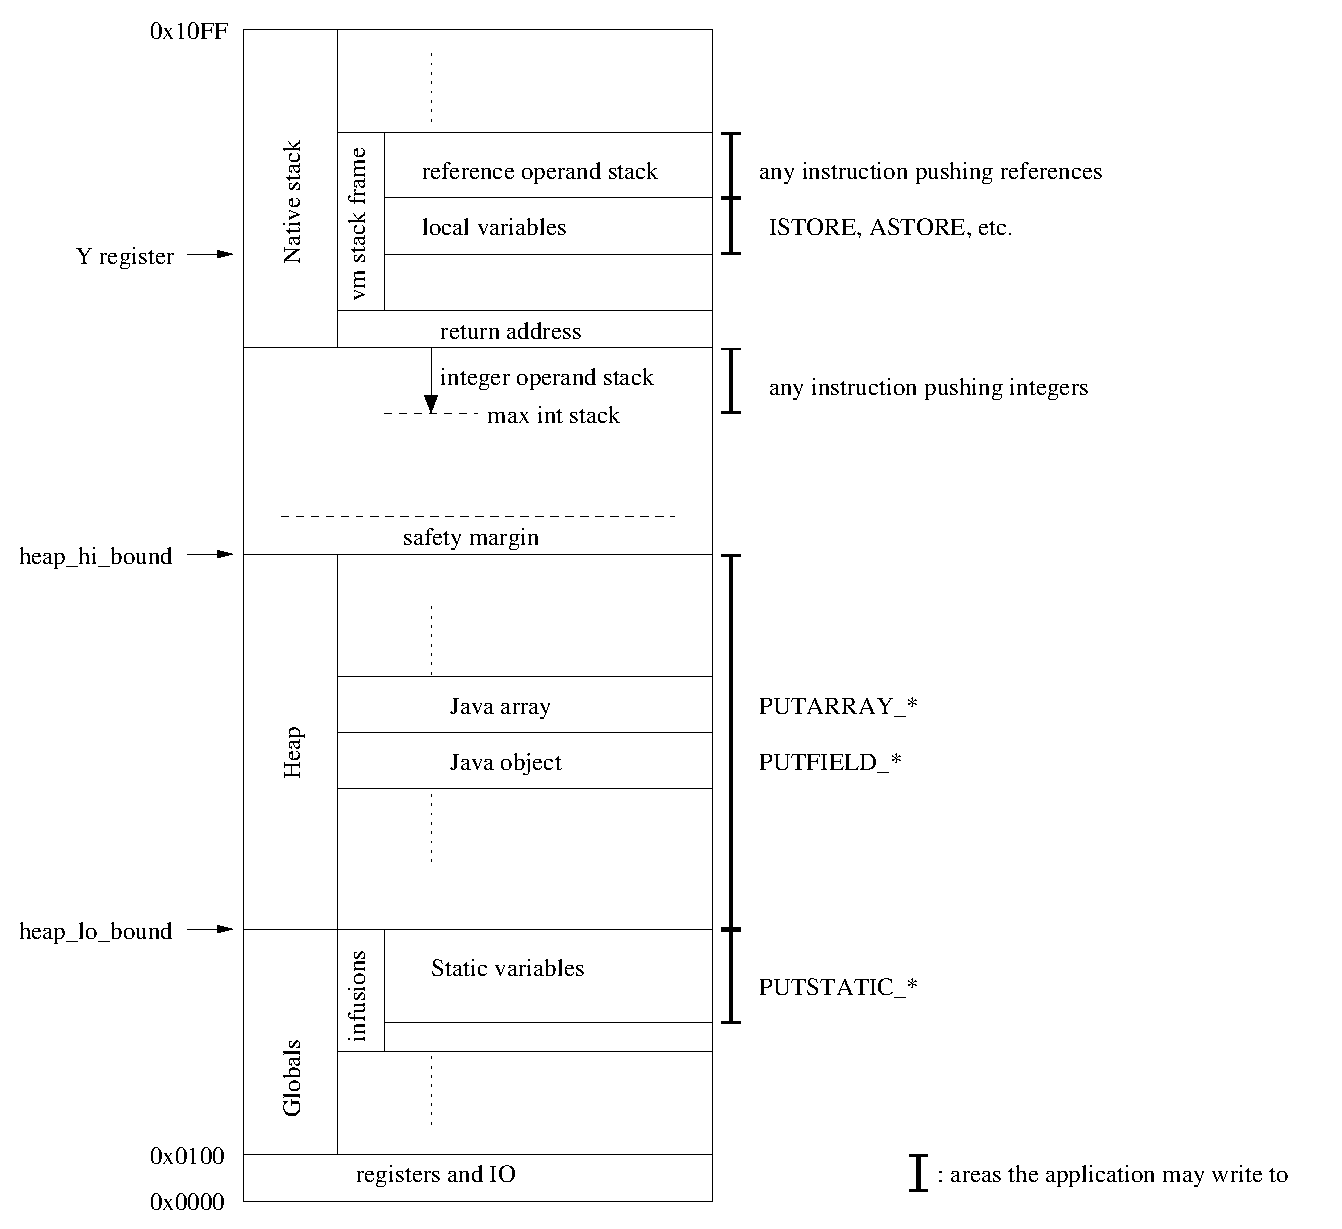
\includegraphics[width=\linewidth]{memlayout.eps}
  \caption{Global memory layout and the areas accessible to the application}
  \label{fig-memlayout}
\end{figure}

Figure \ref{fig-memlayout} shows the global layout of the VM's memory. At the bottom are the internal state of by the VM, stored in a number of global variables, and a block with static variables for each infusion. The infusion blocks are actually allocated on the heap at application startup time, but this part of the heap is then separated from the range the application may use to protect them from bad heap writes. This is followed by the application heap, which contains Java objects and arrays.

The native stack grows down in memory towards the heap. This contains a mix of native stack frames for internal VM functions, the application's JVM stack frames containing space for local variables and reference operand stack, and the integer operand stack which grows down directly on top of the native stack.

Thus, the VM's private data and the application data are mixed in the node's memory. The application is only allowed to write to the areas indicated with bars to the right. Any write outside of these designated areas may corrupt the VM's internal state, and needs to be prevented by our safety checks.

Having ensured control flow safety, we can now rely on the fact that we will always execute complete JVM instructions, and the application cannot skip past an inserted run-time check by jumping to the middle of a generated instruction. This means we can demonstrate memory safety by considering each how each JVM instruction writes to memory, and showing they are all either guaranteed to write to a correct address, or checked at run-time. Again, we group instructions in the categories shown below with respect to their writes to memory, as shown in Table \ref{tbl-memory-write-instructions}, and consider each separately.

\begin{table}
\caption{Instructions writing to memory}
\label{tbl-memory-write-instructions}
    \begin{tabular}{ll}
    \toprule
    Type                                 & Writes to \\
    \midrule
    \midrule
    \mycode{STORE}s                      & A local variable in the current method's stack frame \\
    \mycode{PUTSTATIC}s                  & A static variable in an infusion \\
    \mycode{PUTARRAY}s                   & An array on the heap \\
    \mycode{PUTFIELD}s                   & An object on the heap \\
    Any instruction pushing to the stack & The reference or integer stack \\
    \bottomrule
    \end{tabular}
\end{table}

The stack frame for a method contains space for its local variables and reference stack, as shown in Figure \ref{fig-memlayout}. For normal methods, the VM creates the stack frame based on the method header, so at load time we know how much space will be available at run-time. Lightweight methods don't create their own stack frame. Instead, they depend on the caller's stack frame, so whenever we translate an \mycode{INVOKELIGHT} instruction, we need to verify the stack frame of the current method has reserved enough free space for the lightweight method's locals and stack (\ref{chk-sufficient-locals-at-invokelight} and \ref{chk-sufficient-stack-space-at-invokelight}). To do this, the method header contains both the total number of slots to reserve, and the number the method will use for itself. Any remaining slots are used for lightweight methods.

\subsection{The operand stack}
The VM will reserve space for the operand stacks based on the information in the method header, so we need to make sure the actual stack depth neither underflows, or exceeds the maximum announced in the header.

The effect of each instruction on the stack is known at translation time. We simply the verification process by requiring the stack to be empty at all branches, so we can determine the stack depth in a single top to bottom pass. Alternatively, we could announce the expected stack state for each branch target in the method header so we can check the state matches at each branch and corresponding branchtarget. However, this is more complex and in practice the overhead for requiring an empty operand stack at branches is minimal: in our entire Java codebase, only four trivial rewrites to avoid the \mycode{? :} operator were necessary.

This allows us to verify the stack simply by maintaining two counters indicating how many values are on the integer and reference stacks, and updating these counters for each instruction's stack effects as we translate the method. For normal methods both counters are initialised to 0, since they start with empty stacks. Lightweight methods start with their parameters on the stack, so when translating these, the counters are initialised according to the number of arguments announced in the method header.

For each translated instruction, we then check there are enough values on the stack to consume its operands (\ref{chk-no-operandstack-underflow}), and we do not exceed the maximum stack depth announced in the header after pushing it's results (\ref{chk-no-operandstack-overflow}).

Most bytecode instructions have a fixed effect on the stack, for example \mycode{IADD} will always consume two 32-bit ints and push another. We encode this in a simple table. Method calls, discussed below, require some more work to determine the stack effects. 

\paragraph{Invoke instructions}
The \mycode{INVOKESTATIC}, \mycode{INVOKESPECIAL}, and \mycode{INVOKELIGHT} instructions all contain the id of the method that will be invoked. Since we already have all method headers available at translation time, which contain the number of arguments and return type, it is easy to determine the stack effects of these invoke instructions.
 
For \mycode{INVOKEVIRTUAL} and \mycode{INVOKEINTERFACE} however, the actual method that will be called depends on the object on the stack at run-time. For these, we determine the stack effects based on the first method implementation that matches the call. For valid code all implementations should have the same signature, and thus the same effect on the stack, but malicious code could try to send an implementation in a subclass that has different stack effects. We therefore add a run-time check (\ref{chk-invokevirtual-stack-effects-match}) that will verify the method that is called at runtime, has the same stack effects as the one used to verify the stack at translation time.

\paragraph{Return instructions}
Note that \mycode{RETURN} instructions don't need any special care. The stack depth in the method is verified using the instruction found in the bytecode. It's possible for a method to break the contract established in the method header, for example by using \mycode{RETURN} instead of \mycode{IRETURN} in a method that should return an int. However, this is still safe as long as the stack is empty after the return instruction, as checked by \ref{chk-stack-is-empty-after-return}.

Because the return value is passed in registers to the calling method, the result of using an incorrect return instruction is that either the return value is discarded, or whatever happens to be in the registers is used as a return value, which may corrupt the application's own state, but not the VM's.

\subsection{\mycode{STORE}}
Local variables are written to using the \mycode{STORE} instructions. Each \mycode{STORE} instruction contains the index of the local variable slot to write to, which makes it easy to verify at translation time.

Local variables are accessed as an offset from the \mycode{Y} register, which is under control of the VM and points to the start of the local variables, as shown in Figure \ref{fig-memlayout}. The method header is used to create the current method's stack frame, or in the case of lightweight methods, to verify any caller has reserved enough slots for the lightweight method's locals.

Since we know how many slots will be available at the \mycode{Y} register, we only need to check at translation time that the index of the local is within the range announced in the method header to make sure we will write to a valid location (\ref{chk-local-variable-slot-exists}).

\subsection{\mycode{PUTSTATIC}}
Static variables are allocated globally at the start of the application based on number of static variables in the \emph{infusion} header. The \mycode{PUTSTATIC} instruction contains a reference to an infusion, and the index of the static variable slot. At translation time, we simply need to check the referenced infusion exists (\ref{chk-static-variable-infusion-exists}), and the index is within the legal range (\ref{chk-static-variable-slot-exists}) for that infusion.

\subsection{\mycode{PUTFIELD} and \mycode{PUTARRAY}}
\label{sec-safety-heap-access}
The final type of memory access is to the heap. The various \mycode{NEW} instructions used to create arrays and objects are safe since they are fully implemented in the VM. Writes to heap memory happen using the \mycode{PUTFIELD} and \mycode{PUTARRAY} instructions, which write to object fields and array elements respectively. 

Since these both work on an object reference, a null reference bug could easily trick the VM to write to the lowest addresses. Since in the AVR, the lowest 32 bytes of the address space are mapped to the CPU's general purpose registers, this can cause very hard to diagnose bugs. Similarly, using a high out-of-bounds index into an array, malicious code could easily gain access to the native stack and, for instance, corrupt return addresses.

In some cases it may be possible to verify of these operations at translation time, but this is hard without extensive analysis that would be too expensive for a sensor node. We therefore add a run-time check when translating these instructions just before doing the final memory access, to check the address is within the heap (\ref{chk-memory-access-within-heap}).

The VM will set the bounds of the heap in two variables: \mycode{heap\_lo\_bound} and \mycode{heap\_hi\_bound} as shown in Figure \ref{fig-memlayout}. Each heap access instruction calculates the address to write in the AVR's \mycode{Z} register. Just before the actual write to the heap, we insert al \mycode{CALL} to the \mycode{heapcheck} function shown in Listing \ref{lst-heap-bounds-check}.

This function checks the address in \mycode{Z} is within these bounds. If it is not, it will jump to the \mycode{illegal\_access\_handler}, allowing the VM to terminate the application. This check will add 22 cycles overhead for each array or object write, and 4 bytes code size overhead for the \mycode{CALL} instruction.

The actual write to the heap is often done by an offset from \mycode{Z} using the AVR's \mycode{STD}, or 'store indirect with displacement' instruction. This allows us to write to a fixed offset of at most 63 bytes from \mycode{Z}. For example, to write to object fields, who's offset within the object is know at translation time, we simply load the object's address into \mycode{Z} and use \mycode{STD} to write to the correct offset.

This means the write could end up at most 63 bytes above the end of the heap. The cheapest way to avoid this would be to not use the \mycode{STD} instruction, but instead use the \mycode{ADIW} to add the offset to \mycode{Z} and use the normal \mycode{ST} instruction to store without displacement. However, this would add 2 bytes and 2 cycles for instruction. Instead we reuse the same small safety margin mentioned in check \ref{chk-no-nativestack-overflow}. This is safe because we will never be writing to a heap object and executing a function in the VM or libc at the same time.

\paragraph{Alternatives}
We considered several alternative implementations for \mycode{heapcheck}. Since the \mycode{CALL} and \mycode{RET} instructions are expensive, we can save 7 cycles by inlining in the check instead of calling it. However, this would increase the code size overhead from 4 bytes to over 30 bytes, which we consider too high.

If we align the top and bottom boundaries of the heap at 256 bytes, this would eliminate the need to bounds check the lower byte of the \mycode{Z} register, \mycode{ZL}. This would save 6 of the 22 cycles, but would waste RAM since some bytes below and above the heap would have to remain unused. Since RAM is such a scarce resource and the performance gain is limited, we decided against this.

Finally, we can save 8 cycles if we keep the bounds in registers instead of memory, which would remove the need for the \mycode{LDS} instructions. However this reduces the performance of the stack cache since it means these registers are not available for stack caching. Which of these affects performance more depends on the code. We evaluate the difference in Section \ref{sec-evaluation-run-time-cost}. Since the option to have the bounds in registers is more complex to implement, thus increasing VM size, we choose to keep the bounds in registers.

\begin{listing}[]
	\centering
 	\begin{minted}{c-objdump}
    heapcheck:
        lds  r0, heap_lo_bound
        cp   ZL, r0
        lds  r0, heap_lo_bound + 1
        cpc  ZH, r0
        brlo illegal_access_handler:
        lds  r0, heap_hi_bound
        cp   r0, ZL
        lds  r0, heap_hi_bound + 1
        cpc  r0, ZH
        brlo illegal_access_handler:
        ret
	\end{minted}
	\caption{Heap bounds check}
	\label{lst-heap-bounds-check}
\end{listing}


%\begin{listing}[H]
%	\centering
% 	\begin{minted}{c-objdump}
%    heapcheck:                               cycles   bytes
%        lds  r0, heap_lo_bound               2        4
%        cp   ZL, r0                          1        2
%        lds  r0, heap_lo_bound + 1           2        4
%        cpc  ZH, r0                          1        2
%        brlo illegal_access_handler:         1        2
%        lds  r0, heap_hi_bound               2        4
%        cp   r0, ZL                          1        2
%        lds  r0, heap_hi_bound + 1           2        4
%        cpc  r0, ZH                          1        2
%        brlo illegal_access_handler:         1        2
%        ret                                  4        2
%	\end{minted}
%	\caption{Heap bounds check}
%	\label{lst-heap-bounds-check}
%\end{listing}

\section{Hardware acceleration}
Sensor node CPUs do not have features such as memory management units (MMUs) and privileged-mode execution used in desktop CPUs. While the added complexity for these cannot be justified in a market driven by extreme pressure to minimise chip cost and area, some more lightweight support from the hardware could significantly reduce the cost of providing safe execution environments, with or without a VM. In this section we consider two possible extensions to the CPU that can be implemented at little cost in terms of chip surface area, and we believe to be generic enough to justify their inclusion in these CPUs.

The two most expensive checks are \ref{chk-no-nativestack-overflow} and \ref{chk-memory-access-within-heap}. The last is the cause of most of the run-time overhead, and both require us to keep a safety margin in between the heap and stack. While this margin is small, RAM memory is a scarce resource we would prefer not to waste.

We propose two checks to be added to the CPU, causing it to trap to a fixed error handler when the check fails to allow the node to terminate the program.

\subsection{Stack overflow protection}
To protect against stack overflow, we propose extending the CPU with a stack bound register. The CPU compares the stack pointer to this stack bound whenever it is modified, either by a direct write or implicitly by a \mycode{PUSH} instruction. If the stack pointer drops below the stack bound, the CPU traps to the error handler.

In our VM, the stack bound register would be set to the value of \mycode{heap\_hi\_bound}, thus eliminating the need for \ref{chk-no-nativestack-overflow}. This is also be a useful safety measure to have for any other embedded code since the low amount of RAM makes stack overflows a real risk in any application, which can lead to unpredictable behaviour and hard to diagnose bugs.

\subsection{Heap write protection}
To eliminate the need to call \mycode{heapcheck} before each write, we propose adding two more registers containing the lower and upper bounds of the area the application is legally allowed to write to. The CPU then checks that writes to memory fall within these bounds, otherwise it traps to the error handler.

The question then becomes which writes should be checked, since the VM should still be able to write to any location, and CPU is not aware of which instructions are part of the VM or part of the application. Several options may be considered here.

\paragraph{Checked store instructions}
The AVR's instruction set contains several blocks of unused opcodes \cite{Atmel:AVRInstructionSetManual}. There is enough space to add checked versions of the 'store indirect with displacement' instruction through register \mycode{Z}, which we use to access the heap. When a store happens using these checked versions, the CPU does the bounds checks, while stores using the unchecked versions can still write to anywhere in memory.

Our VM could then use these checked versions when generating code for \mycode{PUTFIELD} and \mycode{PUTARRAY} to implement \ref{chk-memory-access-within-heap} at no runtime cost, and use the unchecked versions for stores that are known to be safe at load-time, such as \mycode{PUTSTATIC}. This would also be useful for native code approaches like Harbor, which normally verifies writes to memory are guarded by a check similar to ours. Instead it may now allow direct stores as well, as long as the checked store instructions are used, and avoid the run-time overhead in these cases.

However, using the majority of the currently unused opcodes for this feature may be too high a price to pay.

\paragraph{Protected mode}
Alternatively, we may add a status bit to the CPU to indicate a protected mode, and use only two unused opcodes for instructions to set or clear this protected mode bit. When the CPU is in protected mode, all stores are required to fall within the heap bounds, while in unprotected mode the entire address range is accessible.

Instead emitting a call to \mycode{heapcheck}, our VM may now protect the stores for \mycode{PUTFIELD} and \mycode{PUTARRAY} by setting and unsetting the protected mode bit. Since these instructions should only take a single cycle, this would reduce the cost of such checks from 22 to just 2 cycles. Similar to the previous case, native code approaches can also benefit by allowing both writes to memory through the existing guard methods, as well as direct stores preceded by the instruction to turn on protected mode.
